\chapter{Elaboració d'una eina automatitzada per a la generació d'atacs en entorns MQTT}
\label{sec:tool}
En aquest apartat es descriu l'eina automatitzada que s'ha desenvolupat per a la generació de datasets de trànsit MQTT que recullen diversos atacs a la infraestructura estudiada. Aquesta eina permet la creació de dades de trànsit de manera eficient i escalable, facilitant així la investigació i el desenvolupament de models de detecció d'intrusions en entorns IoMT.

Aquesta eina està programada en bash (codi: \ref{lst:tool}), totes les seves funcionalitats són implementades mitjançant contenidors Docker per tal que pugui ser desplegada en qualsevol entorn. Aquesta permet tant el desplegament d'una infraestructura simulada de clients MQTT com la generació dels diferents atacs estudiats en aquest treball de forma automatitzada.

L'eina consta de diversos apartats, que amb la utilitat "getopts" seleccionem els diversos atacs que volem generar mitjançant flags.

El pas inicial és el desplegament d'un contenidor Docker amb imatge base zeek/zeek (basada en linux) \cite{zeekimg} anomenat "sniffer", que desplega un servei de \textit{tcpdump} escoltant la interfície de xarxa del host especificada per l'usuari. Aquest contenidor captura el trànsit benigne i maliciós generat pels atacs i els clients, que desa en un fitxer en format pcap per a ser analitzat posteriorment.

Seguidament, es despleguen els diferents atacs. El primer d'ells és la realització dels atacs de reconeixement de la infraestructura vistos a l'apartat \ref{sec:Recon}. Primer de tot desplega un contenidor Docker amb la imatge base Kali-Linux-Last-Relesase anomenat "escaner" que realitza els atacs enfocats a indentificar la IP del broker que es guarda en una variable d'entorn, seguit dels atacs de descobriment de clients MQTT que guarda en els un arxiu txt. Aquest contendior, finalment, realitza els atacs de descobriment de la informació del broker amb les eines MQTTSA i scripts NSE d'NMAP.

El següent atac implementat és l'atac de denegació de servei distribuït (DDoS) explicat a \ref{fig:DDoS}. Per a aquest atac, es necessiten trobar les IPs lliures de la xarxa per a desplegar clients MQTT maliciosos. Per això, mitjançant l'ús de la utilitat "prips" que ens permet fer càlculs de xarxa i utilitzant la llista de clients trobada en els atacs de reconeixement, es generen una llista de les següents IPs lliures necessàries (a partir de la 100 per mitigar conflictes amb futures assignacións de IP amb DHCP), que es guarden en variables d'entorn. Amb aquestes IPs es desplega mitjançant l'orquestrador "Docker Compose" un seguit de contenidors Docker basats la imatge de kalilinux/kali-last-release que mitjançant l'eina MQTT-Malaria realitzen l'atac de denegació de servei distribuït a la IP del broker trobada i enregistrada anteriorment. Aquest atac es realitza amb un nombre de clients configurables per l'usuari, que s'especifica mitjançant un paràmetre de l'eina.

També, s'implementa l'atac de Man In The Middle (MITM) explicat a \ref{sec:MITM}. Per a això, es desplega un contenidor Docker amb la imatge base Kalilinux/Kali-Last-Release anomenat "spoofer" que realitza l'atac d'ARP spoofing bidireccional entre el broker trobat i un client seleccionat mitjançant l'eina arpspoof. Paral·lelament, es desplega un altre contenidor Docker similar amb les configuracions de ip forwarding i iptables necessàries anomenat "mitm" que executa l'eina mitmproxy, que actua fa que el host atacant actuï com a proxy transparent entre els dos dispositius atacats.

Un cop acabada l'execució i es decideix al finalització per part de l'usuari, l'eina atura tots els contenidors Docker desplegats i fa una avaluació del trànsit generat mitjançant l'IDS zeek ( \ref{sec:Zeek} ). Si bé aquest apartat no és necessari per a la generació del dataset, és d'utilitat per a poder analitzar el funcionament dels atacs i la seva efectivitat, així com per a identificar possibles millores en la implementació d'aquests.

  \begin{figure}[H]
    \centering
    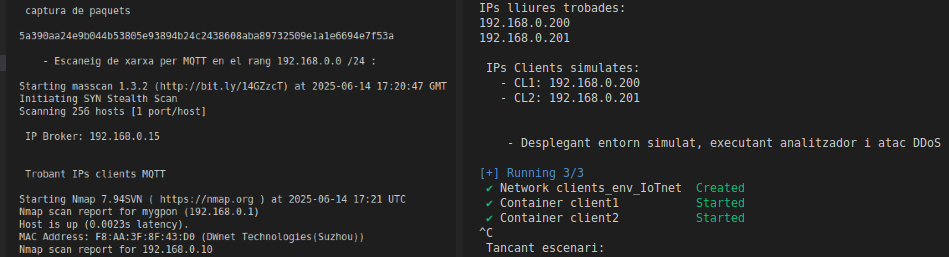
\includegraphics[width=1\textwidth]{img/tool.png}
    \caption{Sortida d'execució de l'eina automatitzada. A l'esquerra es pot veure una part de la sortida dels atacs de reconeixement mentre que a la dreta la sortida dels atacs de DDoS.}
    \label{fig:tool}
  \end{figure}


\